\documentclass[spanish,mexico]{beamer}
\usetheme{metropolis}           % Use metropolis theme
% Packages
% Speakers will often include extra slides at the end of their presentation to refer to during audience questions. One easy way to do this is to include the appendixnumberbeamer package in your preamble and call \appendix before your backup slides
\usepackage{appendixnumberbeamer}
\usepackage{babel} % We speak español
% You should load babel or polyglossia before biblatex and
% then biblatex will detect babel or polyglossia automatically.
\usepackage[url=false]{biblatex}
\addbibresource{references.bib}
% When using the hyperref package, it is preferable to load it after biblatex.
\usepackage{booktabs} % To get nice looking tables
%\usepackage{hyperref} % Loaded by default while using the beamer class, so we have to use the next command
\hypersetup{
	bookmarks=true,          % show bookmarks bar?
	%unicode=false,          % non-Latin characters in Acrobat’s bookmarks
	%pdftoolbar=true,        % show Acrobat’s toolbar?
	%pdfmenubar=true,        % show Acrobat’s menu?
	%pdffitwindow=false,     % window fit to page when opened
	%pdfstartview={FitH},    % fits the width of the page to the window
	%pdftitle={My title},    % title
	%pdfauthor={Author},     % author
	%pdfsubject={Subject},   % subject of the document
	%pdfcreator={Creator},   % creator of the document
	%pdfproducer={Producer}, % producer of the document
	%pdfkeywords={keyword1, key2, key3}, % list of keywords
	%pdfnewwindow=true,      % links in new PDF window
	colorlinks=true,       	 % false: boxed links; true: colored links. 
	linkcolor=black,         % color of internal links (change box color with linkbordercolor)
	%citecolor=green,        % color of links to bibliography
	%filecolor=cyan,         % color of file links
	urlcolor=magenta         % color of external links. 
	% IMPORTANT:
	% Options from here (https://en.wikibooks.org/wiki/LaTeX/Hyperlinks#Customization). 
	% If colorlinks=true, then all kinds of links get colored.
	% linkcolor value was changed from red to black. Try with red to see the difference.
}
\usepackage{listings} % add lstlisting environment
\title{Plantilla para beamer}
\date{\today}
\author{Francisco Murphy Pérez}
\institute{Instituto de Biotecnología - Universidad Nacional Autónoma de México}
\begin{document}
	\maketitle
	\section{Primera parte}
	\begin{frame}{¿Por qué?}
		Porque$\ldots$
		\begin{itemize}
			\item Necesito una plantilla lista para usar.
			\item Tengo que aprender a usar mejor \texttt{Beamer}.
		\end{itemize}
	\end{frame}
	\begin{frame}{¿Por qué no en Rstudio/Quarto/Revealjs?}
		\begin{enumerate}
			\item Por razones secretas.
			\item Porque la alternativa no es lo suficientemente estable.
			\item Tengo experiencia en \LaTeX{}.
		\end{enumerate}
	\end{frame}
	\begin{frame}[fragile]{Requisitos}
		Se supone que el tema se ve mejor con esta \href{https://mozilla.github.io/Fira/}{fuente}.
		En Fedora, esto se resuelve al ingresar el siguiente comando en una terminal:\\
		%\begin{lstlisting}
		%sudo dnf install mozilla-fira-*
		%\end{lstlisting}
		% If in the output you get some strange characters
		% Use: lstlisting with gobble 
		%\begin{lstlisting}[gobble=6]
		%sudo dnf install mozilla-fira-*
		%\end{lstlisting}
		% OR
		% Use: lstinputlisting, without spaces
		\lstinputlisting{cmdline.sh}
	\end{frame}
	\section{Segunda parte}
	\begin{frame}{Matemáticas}
		La fórmula para obtener la distancia entre dos puntos A y B, con coordenadas \((x_1, y_1)\) y \((x_2, y_2)\), respectivamente, es 
		\begin{equation}
		d=\pm\sqrt{(x_{2}-x_{1})^2+(y_{2}-y_{1}^2)}
		\end{equation}
		
		Para obtener las coordenadas del punto medio M, con coordenadas \((x_\mathrm{m}, y_\mathrm{m})\),  entre dos puntos A y B, con coordenadas \((x_1, y_1)\) y \((x_2, y_2)\), respectivamente, tenemos que:
		\begin{align}
			x_\mathrm{m} = \frac{x_1+x_2}{2} \\
			y_\mathrm{m} = \frac{y_1+y_2}{2} 
		\end{align}
	\end{frame}
		\begin{frame}{Imágenes, tablas y dos columnas}
		\begin{columns}
			\column{0.5\textwidth}
			\begin{figure}
				\caption{Imagen tomada de \href{https://www.picpng.com/linux-unix-tux-penguin-cute-png-43298}{aquí}.}
				\centering
				
\includegraphics[width=0.5\textwidth]{tux}
			\end{figure}
			\column{0.5\textwidth}
			\begin{table}[]
				\begin{tabular}{@{}llr@{}}
					\toprule
					\multicolumn{2}{c}{Item} &            \\ \midrule
					Animal     & Description & Price (\$) \\ \midrule
					Gnat       & per gram    & 13.65      \\
					& each        & 0.01       \\
					Gnu        & stuffed     & 92.50      \\
					Emu        & stuffed     & 33.33      \\
					Armadillo  & frozen      & 8.99       \\ \bottomrule
				\end{tabular}
				\caption{Ejemplo tomado de \href{https://www.tablesgenerator.com/}{acá}.}
				\label{tab:my-table}
			\end{table}
		\end{columns}
	\end{frame}
	\begin{frame}{Gráficas}
		% Por el momento las gráficas se hacen con ggplot2
		% y se importan aquí.
		% TODO: \usepackage{graphicx} required
		\begin{figure}[h]
			\centering
			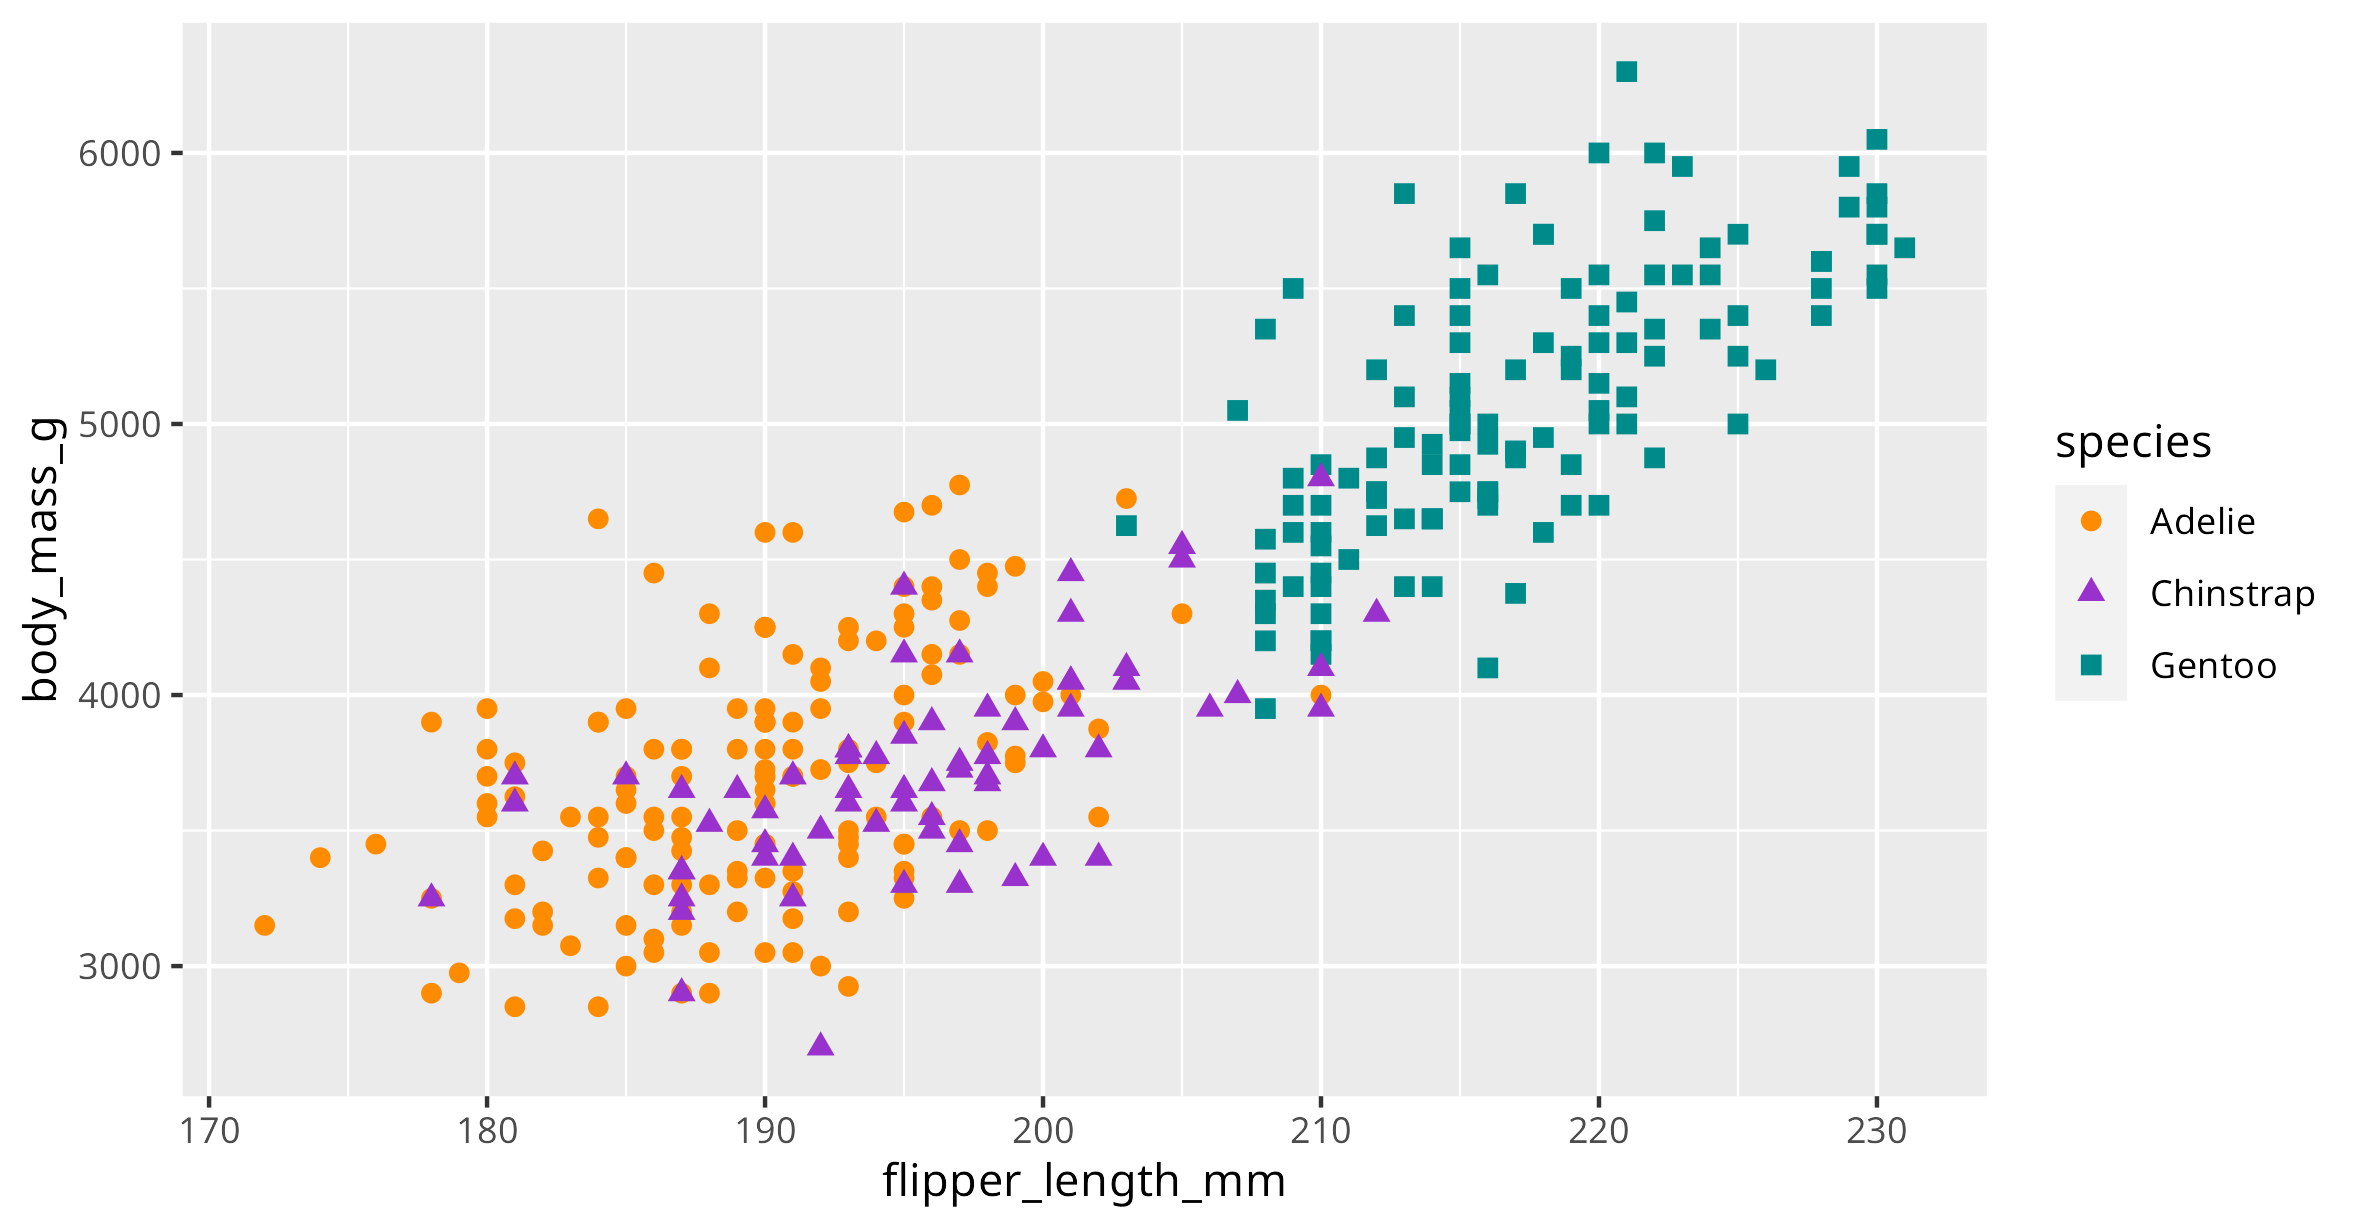
\includegraphics[width=0.9\linewidth]{plot}
			\caption{Datos tomados del paquete \href{https://education.rstudio.com/blog/2020/07/palmerpenguins-cran/\#the-palmerpenguins-package}{palmerpenguins}.}
			\label{fig:plot}
		\end{figure}
	\end{frame}
	\begin{frame}{Bloques}
	\begin{theorem}
		Teorema
	\end{theorem}
	\begin{example}
		Ejemplo
	\end{example}
	\begin{proof}
		Demostración
	\end{proof}
	\begin{corollary}
		Corolario
	\end{corollary}
	\begin{lemma}
		Lema
	\end{lemma}
\end{frame}
\begin{frame}{Citas}
	Este es un ejemplo de cita \cite{Agnarelli2021} y otro con múltiples citas \cite{Burla2020,Dodson2021,Greisman2022,Hatti2021,Joshua2020}.
\end{frame}
\begin{frame}{Películas}
	content...
\end{frame}
\section{Conclusiones}
\begin{frame}{Conclusión}
	En conclusión$\ldots$
\end{frame}
\appendix
\begin{frame}[allowframebreaks]{Bibliografía}
	\printbibliography[heading=none]
\end{frame}
\end{document}